\subsection{Experiment 2: Static fabrics vs. Dynamic fabrics}%
\label{sub:experiment_2_static_fabrics_vs_dynamic_fabrics}

In motion planning for dynamic environments, global and local planning methods work together
to achieve efficient and safe motion of the robot. However, \ac{sf}
are not designed to follow global paths. Path
following can only be achieved using a pseudo-dynamic approach where the forcing potential
is shifted in every time step without considering the dynamics of the trajectory.
Therefore, we
propose \ac{df} to allow smoother path following tasks, where the speed of
the goal is also considered during execution. 
In this second experiment, we investigate
how \ac{df} compare to \ac{sf} for path following tasks.
Specifically, we show that \ac{df} outperform \ac{sf} when
following a path generated by a global planner.

\paragraph{Simulation}
We evaluated \ac{df} on the \panda{} robot in simulation with an
analytic, time-parameterized curve and a path generated by a global planner, namely RRT
(\cref{fig:experiment2_simPanda_spline_example}).
In the case of the analytic trajectory, the three obstacles were
randomized across all runs. For the experiment with the global planner, the goal position and 
the obstacles were randomized across all runs.
A total of $N=50$ experiments were executed for this
experiment. The reduced summed error for dynamic fabrics verifies the
theoretical finding that dynamic fabrics can follow paths more closely.
The average error over all runs with the
analytic trajectory is $0.0792$m (\ac{df})
and $0.136$m (\ac{sf}), see
\cref{subfig:experiment2_simPanda_res_analytic} for the comparison.
For the spline path generated with RRT, the
average error over all runs is $0.145$m (\ac{df}) and $0.240$m (\ac{sf}), see
\cref{subfig:experiment2_simPanda_res_spline} for the comparison.


\begin{figure}[h]
  \begin{subfigure}{0.5\linewidth}
    \centering
    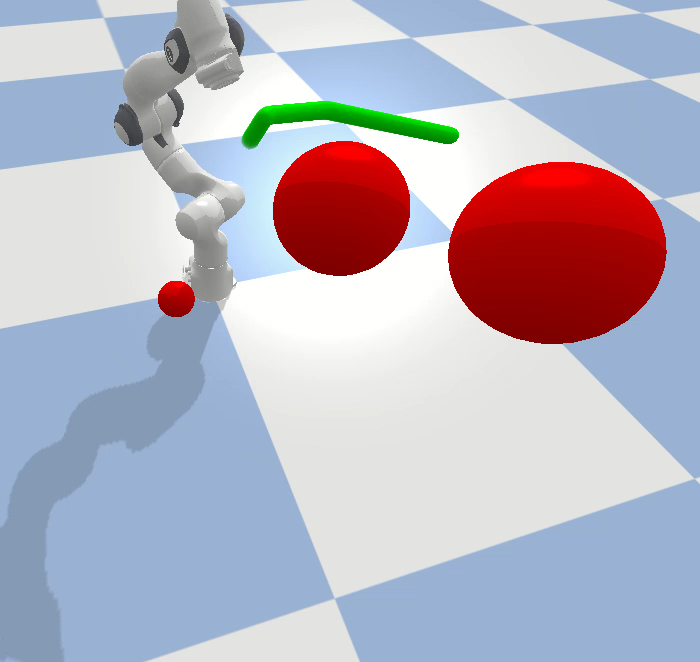
\includegraphics[width=0.95\textwidth]{2_static_dynamic/simPanda/spline/dynamic_fabrics_rrt_1.png}
  \end{subfigure}%
  \begin{subfigure}{0.5\linewidth}
    \centering
    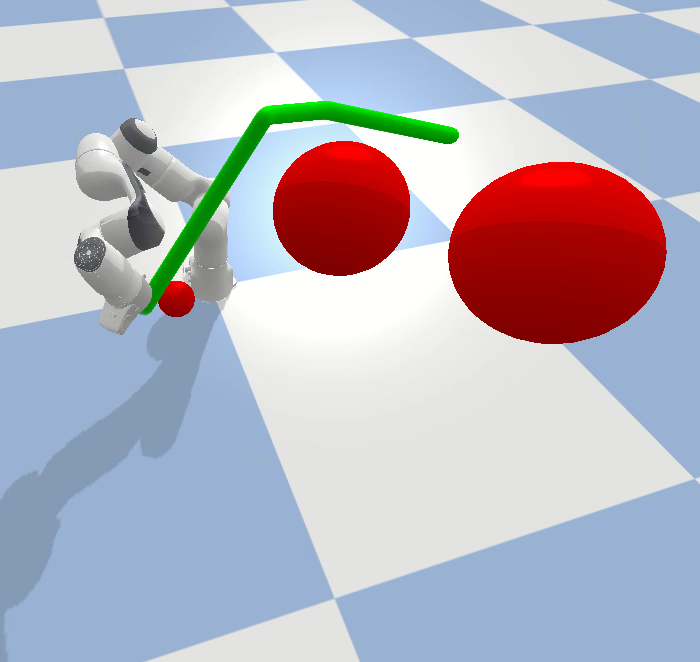
\includegraphics[width=0.95\textwidth]{2_static_dynamic/simPanda/spline/dynamic_fabrics_rrt_2.png}
  \end{subfigure}
  \caption{Path generated with RRT from OMPL.}
  \label{fig:experiment2_simPanda_spline_example}
\end{figure}

\begin{figure}[h]
  \begin{subfigure}{0.5\linewidth}
    \centering
    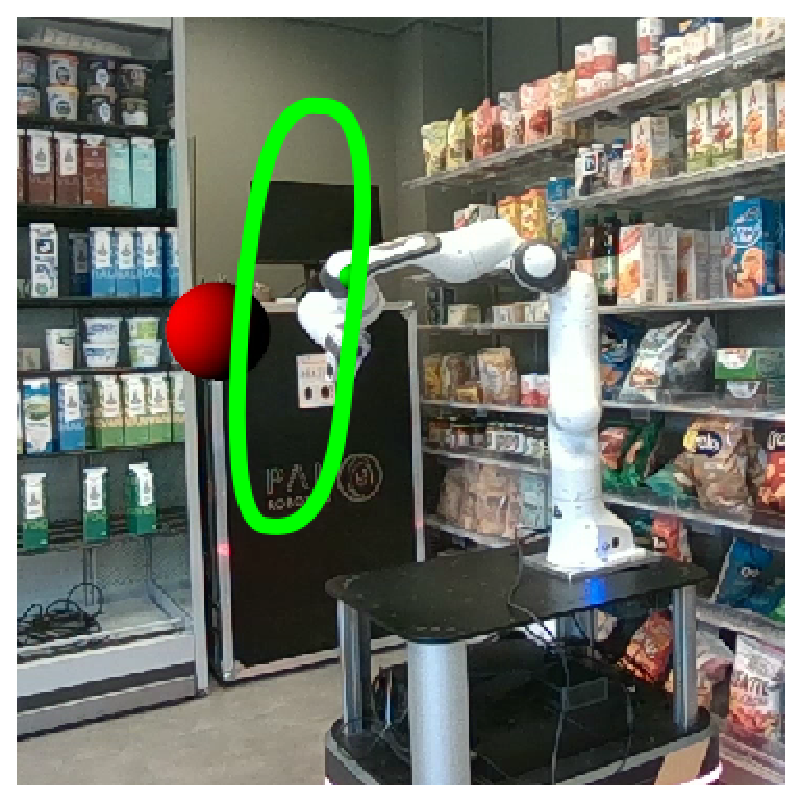
\includegraphics[width=0.95\textwidth]{2_static_dynamic/realPanda/2_static_dynamic_example_analytic}
    \caption{}
  \end{subfigure}%
  \begin{subfigure}{0.5\linewidth}
    \centering
    
\includegraphics[width=0.95\textwidth]{2_static_dynamic/realPanda/2_static_dynamic_example_spline}
    \caption{}
  \end{subfigure}
  \caption{Trajectory following tasks with \acl{df}. In (a), the trajectory is a 
  time-parameterized analytic curve. In (b), the trajectory is described by a spline.}%
  \label{fig:experiment2_realPanda_examples}
\end{figure}




\begin{figure}[h]
  \centering
  \begin{subfigure}{1.0\linewidth}
    \centering
    \includegraphics[angle=-90,width=\textwidth]{2_static_dynamic/simPanda/analytic/results_comparison}
    \caption{Analytic, user-specified global path}%
    \label{subfig:experiment2_simPanda_res_analytic}
  \end{subfigure}
  \begin{subfigure}{1.0\linewidth}
    \centering
    \includegraphics[angle=-90,width=\textwidth]{2_static_dynamic/simPanda/spline/results_comparison}
    \caption{Global path generated by RRT using OMPL}%
    \label{subfig:experiment2_simPanda_res_spline}
  \end{subfigure}
  \caption{Comparison between static and dynamic fabrics for trajectory following tasks
    in simulation. Lower values in a metric indicate that \ac{df} performed better than
    \ac{sf}.
  }%
  \label{fig:experiment2_simPanda}
\end{figure}

\paragraph{Real-World}
Path following was also assessed with the real \panda{} in similar settings.
Quantitative results are only presented for $N=20$ different paths with splines
where up to three obstacles were added to the workspace, see \cref{fig:experiment2_realPanda_examples}. The results in real-world confirm the 
findings from the simulation. By exploiting the velocity information of the 
trajectory, the integration error can be effectively
reduced, \cref{fig:experiment2_realPanda_res}. In contrast to the simulation
we see a higher fluctuation in solver times, which can be caused by a generally lower capacity 
of the computing unit on the robot.

\begin{figure}[h]
    \centering
    \includegraphics[angle=-90,width=\linewidth]{2_static_dynamic/realPanda/results_comparison}
    \caption{Comparison between \ac{sf} and \ac{df} when following a path defined
      by a basic spline in the real world. 
      The splines and the obstacles are different for the $N=20$ case.
      \ac{df} achieve lower deviation errors that \ac{sf}.
    }%
    \label{fig:experiment2_realPanda_res}
\end{figure}



